\subsection{蛇形图}

命题 1. 考虑交换群的一个交换图：

\[
\begin{array}{c c c} \mathrm{A} & \xrightarrow {u} & \mathrm{B} \\ a \Big \downarrow & & b \Big \downarrow \\ \mathrm{A} ^ {\prime} & \xrightarrow {} u ^ {\prime} & \mathrm{B} ^ {\prime} \end{array} \xrightarrow {v} \begin{array}{c c c} \mathrm{C} \\ c \Big \downarrow \\ \mathrm{C} ^ {\prime} \end{array}\tag{10}
\]

假设 (10) 的两行都是正合的。那么：

\begin{enumerate}
\def\labelenumi{(\roman{enumi})}
\tightlist
\item
  若 \(c\) 是单射，我们有
\end{enumerate}

\[
\operatorname{Im} (b) \cap \operatorname{Im} (u ^ {\prime}) = \operatorname{Im} (u ^ {\prime} \circ a) = \operatorname{Im} (b \circ u).\tag{11}
\]

\begin{enumerate}
\def\labelenumi{(\roman{enumi})}
\setcounter{enumi}{1}
\tightlist
\item
  若 \(a\) 是满射，我们有
\end{enumerate}

\[
\operatorname{Ker} (b) \dot {+} \operatorname{Im} (u) = \operatorname{Ker} (v ^ {\prime} \circ b) = \operatorname{Ker} (c \circ v).\tag{12}
\]

我们证明 (i)。显然

\[
\operatorname{Im} (u ^ {\prime} \circ a) = \operatorname{Im} (b \circ u) \subset \operatorname{Im} (b) \cap \operatorname{Im} (u ^ {\prime}).
\]

反之，设 \(x \in \operatorname{Im}(b) \cap \operatorname{Im}(u')\) 。存在 \(y \in B\) 使得 \(x = b(y)\) 。由于 \(v' \circ u' = 0\) ，我们有 \(0 = v'(x) = v'(b(y)) = c(v(y))\) ，由此得 \(v(y) = 0\) （因 \(c\) 是单射）。由于 \((u, v)\) 是正合列，存在 \(z \in A\) 使得 \(y = u(z)\) ，从而 \(x = b(u(z))\) 。

我们证明 (ii)。由于 \(v \circ u = 0\) 且 \(v' \circ u' = 0\) ，显然

\[
\operatorname{Ker} (b) + \operatorname{Im} (u) \subset \operatorname{Ker} (v ^ {\prime} \circ b) = \operatorname{Ker} (c \circ v).
\]

反之，设 \(x \in \operatorname{Ker}(v' \circ b)\) 。则 \(b(x) \in \operatorname{Ker}(v')\) ，且存在 \(y' \in A'\) 使得 \(u'(y') = b(x)\) （因序列 \((u', v')\) 正合）。由于 \(a\) 是满射，存在 \(y \in A\) 使得 \(a(y) = y'\) ，从而 \(b(x) = u'(a(y)) = b(u(y))\) ；由此得 \(x - u(y) \in \operatorname{Ker}(b)\) ，这样就完成了证明。

引理 1. 考虑交换群的一个交换图：

\[
\begin{array}{c} \mathrm{A} \xrightarrow {u} \mathrm{B} \\ a \Big \downarrow \\ \mathrm{A} ^ {\prime} \xrightarrow [ u ^ {\prime} ]{} \mathrm{B} ^ {\prime} \end{array}\tag{13}
\]

则存在一个且仅一个同态 \(u_1 \colon \operatorname{Ker}(a) \to \operatorname{Ker}(b)\) ，以及一个且仅一个同态 \(u_2 \colon \operatorname{Coker}(a) \to \operatorname{Coker}(b)\) ，使得诸图

\begin{enumerate}
\def\labelenumi{(\arabic{enumi})}
\setcounter{enumi}{13}
\tightlist
\item
\end{enumerate}

和

\pandocbounded{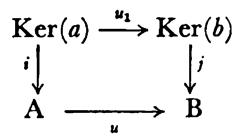
\includegraphics[keepaspectratio]{images/part001_d47c3bb2.jpg}}

\begin{enumerate}
\def\labelenumi{(\arabic{enumi})}
\setcounter{enumi}{14}
\tightlist
\item
\end{enumerate}

\pandocbounded{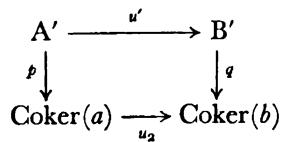
\includegraphics[keepaspectratio]{images/part001_9d56bddd.jpg}}

都是交换的，其中 \(i\) 和 \(j\) 表示典范单射， \(p\) 和 \(q\) 表示典范满射。

若 \(x \in \operatorname{Ker}(a)\) ，则 \(a(x) = 0\) 且 \(b(u(x)) = u'(a(x)) = 0\) ，因此 \(u(x) \in \operatorname{Ker}(b)\) ，于是 \(u_1\) 的存在性和唯一性是直接的。类似地，我们有 \(u'(a(A)) = b(u(A)) \subset b(B)\) ，然后取商， \(u'\) 给出一个同态 \(u_2\) ： \(\operatorname{Coker}(a) \to \operatorname{Coker}(b)\) ，它是使 (15) 交换的唯一的同态。

现在从交换群交换图 (10) 出发；由引理 1，与它对应有一个图

\begin{enumerate}
\def\labelenumi{(\arabic{enumi})}
\setcounter{enumi}{15}
\tightlist
\item
\end{enumerate}

\pandocbounded{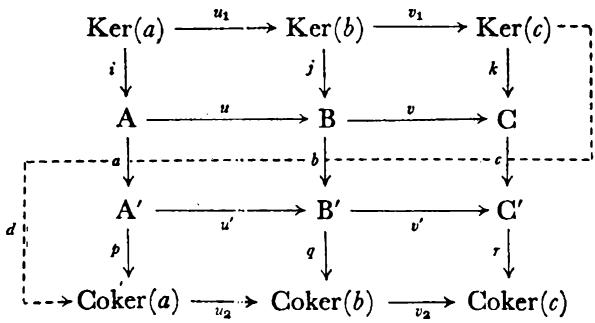
\includegraphics[keepaspectratio]{images/part001_af6ee28a.jpg}}

其中 \(i, j, k\) 是典范单射， \(p, q, r\) 是典范满射，而 \(u_{1}, u_{2}\) （相应地 \(v_{1}, v_{2}\) ）是由引理 1 典范地伴随于 \(u, u'\) （相应地 \(v, v'\) ）的同态。立即可验证这个图是交换的。

命题 2. 假设在交换图 (10) 中，序列 \((u, v)\) 和 \((u', v')\) 都是正合的。那么：

\begin{enumerate}
\def\labelenumi{(\roman{enumi})}
\item
  \(v_{1} \circ u_{1} = 0\) ；若 \(u'\) 是单射，则序列 \((u_{1}, v_{1})\) 正合。
\item
  \(v_{2} \circ u_{2} = 0\) ；若 \(v\) 是满射，则序列 \((u_{2}, v_{2})\) 正合。
\item
  假设 \(u'\) 是单射且 \(v\) 是满射。则存在一个且仅一个同态 \(d: \operatorname{Ker}(c) \to \operatorname{Coker}(a)\) ，它具有下列性质：若 \(x \in \operatorname{Ker}(c)\) ， \(y \in B\) 和 \(t' \in A'\) 满足关系 \(v(y) = k(x)\) 和 \(u'(t') = b(y)\) ，则 \(d(x) = p(t')\) 。此外，序列
\end{enumerate}

\[
(*) \quad \operatorname{Ker} (a) \xrightarrow {u _ {1}} \operatorname{Ker} (b) \xrightarrow {v _ {1}} \operatorname{Ker} (c) \xrightarrow {d}
\]

\[
\operatorname{Coker} (a) \xrightarrow {u _ {2}} \operatorname{Coker} (b) \xrightarrow {v _ {2}} \operatorname{Coker} (c)
\]

是正合的。

我们证明 (i)。由于 \(u_{1}\) 和 \(v_{1}\) 分别与 \(u\) 和 \(v\) 在 \(\operatorname{Ker}(a)\) 和 \(\operatorname{Ker}(b)\) 上的限制有相同的图，我们有 \(v_{1} \circ u_{1} = 0\) 。于是

\[
\operatorname{Ker} (v _ {1}) = \operatorname{Ker} (b) \cap \operatorname{Ker} (v) = \operatorname{Ker} (b) \cap \operatorname{Im} (u) = \operatorname{Im} (j) \cap \operatorname{Im} (u).
\]

但是，由命题 1 (i)，有 \(\operatorname{Ker}(v_1) = \operatorname{Im}(j \circ u_1) = \operatorname{Im}(u_1)\) （若 \(u'\) 是单射）。

我们证明 (ii)。由于 \(u_{2}\) 和 \(v_{2}\) 是由 \(u\) 和 \(v\) 取商得到的，显然 \(v_{2} \circ u_{2} = 0\) 。设 \(v\) 是满射；由于 \(q\) 和 \(p\) 是满射，由诸假设和命题 1 (ii) 得

\[
\begin{array}{r l} \operatorname{Ker} (v _ {2}) & = q (\operatorname{Ker} (v _ {2} \circ q)) = q (\operatorname{Ker} (v ^ {\prime}) + \operatorname{Im} (b)) = q (\operatorname{Ker} (v ^ {\prime})) = q (\operatorname{Im} (u ^ {\prime})) \\ & = \operatorname{Im} (q \circ u ^ {\prime}) = \operatorname{Im} (u _ {2} \circ p) = \operatorname{Im} (u _ {2}). \end{array}
\]

最后证明 (iii)。对 \(x \in \operatorname{Ker}(c)\) ，存在 \(y \in B\) 使得 \(v(y) = k(x)\) （因 \(v\) 是满射）；此外 \(v'(b(y)) = c(k(x)) = 0\) ，因而存在唯一的 \(t' \in A'\) 使得 \(u'(t') = b(y)\) （因 \(u'\) 是单射）。我们现在证明，元素 \(p(t') \in \operatorname{Coker}(a)\) 不依赖于元素 \(y \in B\) （只要 \(v(y) = k(x)\) ）。因为若 \(y' \in B\) 是另一个满足 \(v(y') = k(x)\) 的元素，则 \(y' = y + u(z)\) ，其中 \(z \in A\) ；我们证明：若 \(t'' \in A'\) 满足 \(u'(t'') = b(y')\) ，则 \(t'' = t' + a(z)\) ；因为

\[
u ^ {\prime} \left(t ^ {\prime} + a (z)\right) = u ^ {\prime} \left(t ^ {\prime}\right) + u ^ {\prime} (a (z)) = b (y) + b (u (z)) = b (y + u (z)) = b \left(y ^ {\prime}\right).
\]

最后，由此得 \(p(t'') = p(t') + p(a(z)) = p(t')\) 。于是可以令 \(d(x) = p(t')\) ，映射 \(d: \operatorname{Ker}(c) \to \operatorname{Coker}(a)\) 就这样被定义了。现在若 \(x_1, x_2\) 是 \(\operatorname{Ker}(c)\) 的元素且 \(x = x_1 + x_2\) ，我们取 B 的元素 \(y_1, y_2\) ，使得 \(v(y_1) = k(x_1)\) 和 \(v(y_2) = k(x_2)\) ，并为 \(y \in B\) 选取元素 \(y_1 + y_2\) ；于是立即可得 \(d(x) = d(x_1) + d(x_2)\) ，因而 \(d\) 是一个同态。

设 \(x = v_{1}(x')\) ，其中 \(x' \in \operatorname{Ker}(b)\) ；于是取 \(y \in B\) 为元素 \(j(x')\) 。由于 \(b(j(x')) = 0\) ，由此得 \(d(x) = 0\) ，因此 \(d \circ v_{1} = 0\) 。反之，设 \(d(x) = 0\) 。在上面的记号下，我们有 \(t' = a(s)\) ，其中 \(s \in A\) 。这时我们有 \(b(y) = u'(t') = u'(a(s)) = b(u(s))\) ，即 \(b(y - u(s)) = 0\) 。因此元素 \(y - u(s)\) 具有 \(j(n)\) 的形式，其中 \(n \in \operatorname{Ker}(b)\) ，并且我们有 \(k(x) = v(y) = v(u(s) + j(n)) = v(j(n)) = k(v_1(n))\) ；由于 \(k\) 是单射， \(x = v_1(n)\) ，这就证明了序列 (*) 在 \(\operatorname{Ker}(c)\) 处正合。

最后，我们有（始终用同一记号）

\[
u _ {2} (d (x)) = u _ {2} \left(p \left(t ^ {\prime}\right)\right) = q \left(u ^ {\prime} \left(t ^ {\prime}\right)\right) = q (b (y)) = 0
\]

因而 \(u_2 \circ d = 0\) 。反之，设 Coker(a) 的一个元素 \(w = p(t')\) 满足 \(u_2(w) = u_2(p(t')) = 0\) （其中 \(t' \in A'\) ）。则 \(q(u'(t')) = 0\) ，因而 \(u'(t') = b(y)\) 对某个 \(y \in B\) 成立；由于 \(v'(u'(t')) = 0\) ，我们有 \(v'(b(y)) = 0\) ，从而 \(c(v(y)) = 0\) ，换句话说， \(v(y) = k(x)\) 对某个 \(x \in \operatorname{Ker}(c)\) 成立，且按定义 \(w = d(x)\) ，这表明序列 (*) 在

Coker(a) 处正合。在 (i) 中已看到它在 \(\operatorname{Ker}(b)\) 处正合，在 (ii) 中它在 \(\operatorname{Coker}(b)\) 处正合，这就完成了 (iii) 的证明。

注记. 如果图 (10) 的群都是某个环 \(\Lambda\) 上的（例如右）模，且诸同态都是 \(\Lambda\) -模同态，则很快可以验证，命题 2 (iii) 中定义的同态 \(d\) 也是一个 \(\Lambda\) -模同态：若 \(x \in \operatorname{Ker}(c)\) 与 \(\alpha \in \Lambda\) ，且 \(y \in B\) 满足 \(v(y) = k(x)\) ，只需注意 \(v(y\alpha) = k(x\alpha)\) 。

推论 1. 假设图 (10) 是交换的且两行都正合。那么：

\begin{enumerate}
\def\labelenumi{(\roman{enumi})}
\item
  若 \(u'\) , \(a\) 和 \(c\) 都是单射，则 \(b\) 是单射。
\item
  若 \(v, a\) 和 \(c\) 都是满射，则 \(b\) 是满射。
\end{enumerate}

断言 (i) 是命题 2 的断言 (i) 的推论：因为 \(\operatorname{Ker}(a) = 0\) 且 \(\operatorname{Ker}(c) = 0\) ，所以 \(\operatorname{Ker}(b) = 0\) 。

断言 (ii) 是命题 2 的断言 (ii) 的推论：因为 \(\operatorname{Coker}(a) = 0\) 且 \(\operatorname{Coker}(c) = 0\) ，所以 \(\operatorname{Coker}(b) = 0\) 。

推论 2. 假设图 (10) 是交换的且两行都正合。在这些条件下：

\begin{enumerate}
\def\labelenumi{(\roman{enumi})}
\item
  若 \(b\) 是单射且 \(a\) 和 \(v\) 是满射，则 \(c\) 是单射。
\item
  若 \(b\) 是满射且 \(c\) 和 \(u'\) 是单射，则 \(a\) 是满射。
\end{enumerate}

为证明 (i)，考虑图

\[
\begin{array}{c c c} u (\mathrm{A}) & \xrightarrow {w} \mathrm{B} & \xrightarrow {v} \mathrm{C} \\ a ^ {\prime} \Big \downarrow & b \Big \downarrow & c \Big \downarrow \\ u ^ {\prime} (\mathrm{A} ^ {\prime}) & \xrightarrow [ w ^ {\prime} ]{} \mathrm{B} ^ {\prime} & \xrightarrow [ v ^ {\prime} ]{} \mathrm{C} ^ {\prime} \end{array}
\]

其中 \(a'\) 是与 b 在 \(u(\mathbf{A})\) 上的限制有相同图的映射，而 w 和 \(w'\) 是典范单射；显然这个图是交换的且它的行是正合的。此外 \(w'\) 是单射，且由假设 v 是满射；于是由命题 2 (iii)，我们有一个正合列

\[
0 = \operatorname{Ker} (b) \longrightarrow \operatorname{Ker} (c) \stackrel {d} {\longrightarrow} \operatorname{Coker} (a ^ {\prime}) = 0
\]

（因 \(b\) 是单射且 \(a'\) 是满射）；由此 \(\operatorname{Ker}(c) = 0\) 。

为证明 (ii)，考虑图

\[
\begin{array}{c} \mathrm{A} \xrightarrow {u} \mathrm{B} \xrightarrow {w} v (\mathrm{B}) \\ a ^ {\prime} \Biggl \downarrow \qquad \qquad b \Biggl \downarrow \qquad \qquad c ^ {\prime} \Biggl \downarrow \\ \mathrm{A} ^ {\prime} \xrightarrow [ w ^ {\prime} ]{} \mathrm{B} ^ {\prime} \xrightarrow [ v ^ {\prime} ]{} v ^ {\prime} (\mathrm{B} ^ {\prime}) \end{array}
\]

其中这次 \(c'\) 是与 c 在 \(v(\mathbf{B})\) 上的限制有相同图的映射，而 \(w\) 和 \(w'\) 分别与 \(v\) 和 \(v'\) 有相同的图；这个图是交换的且它的行是正合的。此外 \(w\) 是满射，且由假设 \(u'\) 是单射；于是由命题 2 (iii)，我们有一个正合列

\[
0 = \operatorname{Ker} (c ^ {\prime}) \xrightarrow {d} \operatorname{Coker} (a) \longrightarrow \operatorname{Coker} (b) = 0
\]

（因 \(b\) 是满射且 \(c'\) 是单射）；由此 Coker \((a) = 0\) 。

